\documentclass[12pt]{article}

\usepackage[a4paper,margin=2.5cm]{geometry}
\usepackage[utf8]{inputenc}
\usepackage[T1]{fontenc}
\usepackage{stix}
\usepackage{fancyhdr}
\usepackage{sectsty}
\usepackage{longtable}
\usepackage{hanging}
\usepackage{multicol}
\usepackage{tabularx}
\usepackage{longtable}
\usepackage{pdflscape}
\usepackage{float}
\usepackage[rightcaption]{sidecap}
\usepackage[table]{xcolor}
\usepackage{listings}
\usepackage{graphicx}
\graphicspath{ {./Images/} }

\newcommand{\fuggveny}{\textbf{A függvények és leírásuk: \\}}
\newcommand{\vonal}{\noindent\rule{\textwidth}{1pt}}


\definecolor{dkgreen}{rgb}{0,0.6,0}
\definecolor{gray}{rgb}{0.5,0.5,0.5}
\definecolor{mauve}{rgb}{0.58,0,0.82}

\lstset{
  language = Java,
  aboveskip = 2mm,
  belowskip = 2mm,
  showstringspaces = false,
  columns = flexible,
  basicstyle = {\small\ttfamily},
  numberstyle = \tiny\color{gray},
  keywordstyle = \color{blue},
  commentstyle = \color{dkgreen},
  stringstyle = \color{mauve},
  breaklines = true,
  breakatwhitespace = true,
  tabsize = 4
}

\pagestyle{fancy}

\begin{document}

\fancyfoot[L]{\textsc{Váradi Richárd Tamás, XA5OZH}}

\begin{titlepage}
  \raggedleft
  \rule{1pt}{\textheight}
  \hspace{0.05\textwidth}
  \parbox[b]{0.75\textwidth}{
    {\Huge\bfseries Programozás alapjai 3. }\\
    [2\baselineskip]
    {\Large\textit{Házi feladat}}\\
    [4\baselineskip]
    {\Large\textsc{Váradi Richárd Tamás}}\\
    [1\baselineskip]
    {\Large\textsc{XA5OZH}}
    \vspace{0.5\textheight}
  }
\end{titlepage}

\section*{\textsc{A feladat ismertetése}}
A feladat, amit választottam ebben a félévben az egy szövegszerkesztő alkalmazás,
amellyel kódokat lehet szerkeszteni. \\
A prgramnak lesz egy olyan grafikus interfésze, amelyet négy féle módon lehet
megváltozatatni:

\begin{multicols}{2}
  \begin{itemize}
    \item Metal
    \item Nimbus
    \item CDE/Motif
    \item GTK+
  \end{itemize}
\end{multicols}

Ezen felül még lehet változtatni a kód színezésének a módját is:
\begin{multicols}{2}
  \begin{itemize}
    \item Eclipse
    \item Default-alt
    \item Default
    \item Dark
    \item Idea
    \item Monokai
    \item Visual Studio
  \end{itemize}
\end{multicols}

Lehet emellett új fájlt létrehozni, menteni, elmenteni máshogy. Aztán vannak még
ilyen szerkesztéshez használatos funkciói is. Ezek rendre a megszokott műveletek:
visszavonás, kivágás, másolás, beillesztés, törlés, keresés, keresés következő,
csere, kijelöl mindent és még az akutális dátumot is betudjuk szúrni. Aztán
tudunk még formátumot változtatni, vagyis lehet tördelni a kódot és lehet állítani
a betűk méretét és stílusát. \\
Maga a szerkesztő felület támogatja a sorok számozását és még az összecsukást is,
ami annyit tesz, hogy ha nagyon sok hasonló kezdetű sor szerepel egymás után,
akkor összelehet őket csukni, hogy ne zavarjanak és ilyenkor eltűnnek, de egy
kis ikon megjelenik az első sora mellett, amellyel újra ki lehet bontani. Ugyan
ez igaz a függvényekre vagy osztályokra is. Ezek mellett még van autómatikus
kiegészítés is.
A szerkesztő az alábbi nyelveknek a szintaxisát tudja kezelni:

\begin{multicols}{3}
  \begin{itemize}
    \item actionscript
    \item asm
    \item bbcode
    \item c
    \item clojure
    \item cpp
    \item cs
    \item css
    \item delphi
    \item dtd
    \item fortran
    \item groovy
    \item html
    \item java
    \item javascript
    \item json
    \item jsp
    \item latex
    \item lisp
    \item lua
    \item makefile
    \item mxml
    \item nsis
    \item perl
    \item php
    \item properties
    \item python
    \item ruby
    \item sas
    \item scala
    \item sql
    \item tcl
    \item unix
    \item vb
    \item bat
    \item xml
  \end{itemize}
\end{multicols}

\section*{\textsc{Use-case}}
\subsection*{\textsc{Diagram}}
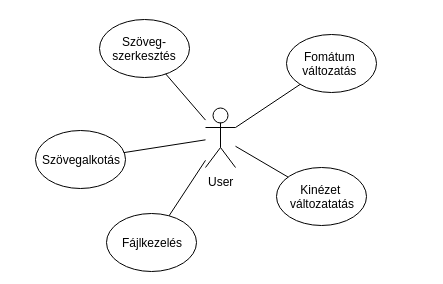
\includegraphics{useCase}

\subsection*{Leírások}
\begin{longtable}[h]{|p{5cm}|p{10cm}|}
  \hline
  \textbf{Cím} & \textbf{Fájlkezelés} \\ \hline
  \textbf{Leírás} & Ezzel tud a felhasználó fájlokat kezelni. \\ \hline
  \textbf{Forgatókönyv} & \textbf{1.} A menübáron menyomva a \textbf{file} pontot
  lenyílik egy fül, amellyel új fájlt tud létrehozni. \\ \hline
  \textbf{Alternatív forgatókönyv} & \textbf{1.A.1} A felhasználó a \textbf{New}
  pontot kiválasztva megtud nyitni egy új fájlt.\\ \hline
  \textbf{Alternatív forgatókönyv} & \textbf{1.A.2} Ha éppen dolgozott valamin a
  felhasználó és azt nem mentette el, akkor felugrik egy ablak, hogy biztos-e
  benne. \\ \hline
  \textbf{Alternatív forgatókönyv} & \textbf{1.B.1} Kitudja választani még az
  \textbf{Open...} pontot is és akkor feljön egy ablak, amin keresztül kitduja
  választani a megnyitandó fájlt. \\ \hline
  \textbf{Alternatív forgatókönyv} & \textbf{1.B.2} Ha éppen dolgozott valamin a
  felhasználó és azt nem mentette el, akkor felugrik egy ablak, hogy biztos-e
  benne. \\ \hline
  \textbf{Alternatív forgatókönyv} & \textbf{1.B.3} Ha meggondolja magát, akkor be
  is tudja zárni az ablakot. \\ \hline
  \textbf{Alternatív forgatókönyv} & \textbf{1.C.1} Eltudja menteni, az aktuális
  munka fájlt a \textbf{Save} ponttal. \\ \hline
  \textbf{Alternatív forgatókönyv} & \textbf{1.C.2} Ha még ez előtt nem volt
  még egyszer sem mentve a fájl, akkor megkérdezi, hogy hova és milyen néven
  szeretnénk menteni. \\ \hline
  \textbf{Alternatív forgatókönyv} & \textbf{1.D.1} Ha a \textbf{Save as...} pontot
  választja, akkor feljön egy olyan ablak, amin keresztül máshova vagy más kiterjesztéssel
  tud fájlokat menteni. \\ \hline
  \textbf{Alternatív forgatókönyv} & \textbf{1.E.1} Ha az \textbf{Exit} pontot
  kiválasztja, akkor bezáródik az alkalmazás. \\ \hline
\end{longtable}

\begin{longtable}[h]{|p{5cm}|p{10cm}|}
  \hline
  \textbf{Cím} & \textbf{Szövegalkotás} \\ \hline
  \textbf{Leírás} & A felhasználónak lesz egy tere, amiben tud szöveg alkotni \\ \hline
  \textbf{Forgatókönyv} & \textbf{1.} A felhasználó belekattint a szövegdobozba
  és elkezd írni \\ \hline
  \textbf{Alternatív forgatókönyv} & \textbf{1.A.1} Ha írásvédett a fájl, akkor
  nem tud beleírni a felhasználó. \\ \hline
\end{longtable}

\begin{longtable}[h]{|p{5cm}|p{10cm}|}
  \hline
  \textbf{Cím} & \textbf{Szövegszerkesztés} \\ \hline
  \textbf{Leírás} & Lehet a szövegben apró módosításokat véghez vinni.\\ \hline
  \textbf{Forgatókönyv} & Lehet visszavonni, szöveg be- és kivinni.\\ \hline
  \textbf{Alternatív forgatókönyv} & \textbf{1.A.1} Vissza tud vonni változtatásokat \\ \hline
  \textbf{Alternatív forgatókönyv} & \textbf{1.B.1} Ki tudja vágni a kijelölt
  szöveget. \\ \hline
  \textbf{Alternatív forgatókönyv} & \textbf{1.C.1} Tud másolni. \\ \hline
  \textbf{Alternatív forgatókönyv} & \textbf{1.D.1} Tud beilleszteni. \\ \hline
  \textbf{Alternatív forgatókönyv} & \textbf{1.E.1} Tud keresni a szövegben. \\ \hline
  \textbf{Alternatív forgatókönyv} & \textbf{1.E.2} Tudja lépteni a keresést. \\ \hline
  \textbf{Alternatív forgatókönyv} & \textbf{1.F.1} Tud cserélni a szövegben. \\ \hline
  \textbf{Alternatív forgatókönyv} & \textbf{1.G.1} Ki lehet jelölni az egész szöveget. \\ \hline
  \textbf{Alternatív forgatókönyv} & \textbf{1.H.1} Betudja szúrni az aktuális dátumot. \\ \hline
\end{longtable}

\begin{longtable}[h]{|p{5cm}|p{10cm}|}
  \hline
  \textbf{Cím} & \textbf{Formátum változtatás} \\ \hline
  \textbf{Leírás} & A szöveg formátumát tudja változtatni. \\ \hline
  \textbf{Forgatókönyv} & Megváltoztatja a szöveget. \\ \hline
  \textbf{Alternatív forgatókönyv} & \textbf{1.A.1} Tudja tördelni a szöveget. \\ \hline
  \textbf{Alternatív forgatókönyv} & \textbf{1.B.1} Tudja változtatni a betűket. \\ \hline
  \textbf{Alternatív forgatókönyv} & \textbf{1.B.2} Lehet a betűkészletet változtatni. \\ \hline
  \textbf{Alternatív forgatókönyv} & \textbf{1.B.3} Lehet a betűstílust váloztatni. \\ \hline
  \textbf{Alternatív forgatókönyv} & \textbf{1.B.4} Lehet a méretet vátoztatni. \\ \hline
\end{longtable}

\begin{longtable}[h]{|p{5cm}|p{10cm}|}
  \hline
  \textbf{Cím} & \textbf{Kinézet változtatás} \\ \hline
  \textbf{Leírás} & A kinézetét a programnak meglehet változtatni. \\ \hline
  \textbf{Forgatókönyv} & Tud választani, hogy a szövegdoboz kinézetén vagy a
  program kinézetén szeretne változtatni. \\ \hline
  \textbf{Alternatív forgatókönyv} & textbf{1.A.1} Tudja változatatni a program
  kinézetét a feladat leírásában található témák között. \\ \hline
  \textbf{Alternatív forgatókönyv} & \textbf{1.A.2} Tudja változtatni a szövegdoboz
  kinézetének szintaxisát a feladat leírásában található témák között. \\ \hline
\end{longtable}

\section*{Osztálydiagram}
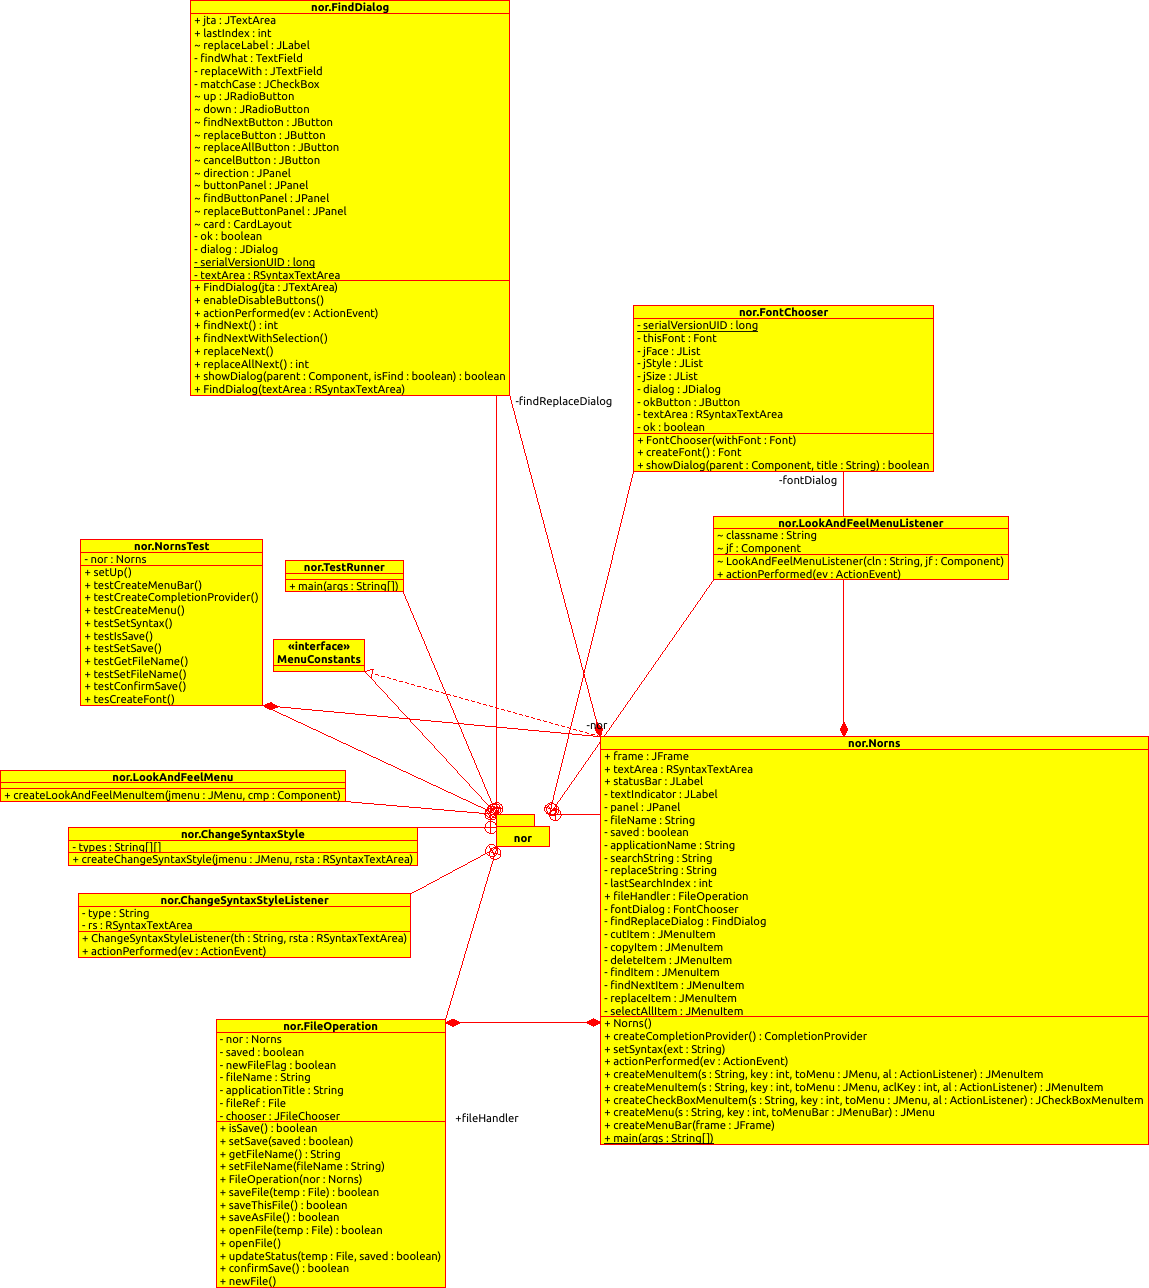
\includegraphics[width = \textwidth]{Uml}
\newpage
\subsection*{Osztályok és interfészek}
\begin{longtable}{|p{5cm}|p{10cm}|} \hline
    \multicolumn{2}{|p{15cm}|}{\textbf{Interfészek}}  \\ \hline
    \textbf{MenuConstants} & Ez lényegében csak egy tároló osztály, amely a menü elemeinek
    a nevét tartalmazza. \\ \hline
\end{longtable}

\begin{longtable}{|p{5cm}|p{10cm}|} \hline
    \multicolumn{2}{|p{15cm}|}{\textbf{Osztályok}}  \\ \hline
    \textbf{FindDialog} & Ezzel lehet létrehozni a keresési ablakot és ebben
    hajtódik végre maga a keresés is.  \\ \hline
    \textbf{FontChooser} & Ezzel lehet létrehozni a betűtípus választási ablakot
    és ebben hajtódik végre maga a logika is. \\ \hline
    \textbf{LookAndFeelMenu} & Ezzel lehet megváltoztatni a program kinézetének
    témáját. \\ \hline
    \textbf{LookAndFeelMenuListener} & Ez figyeli, hogy milyen témát választottunk
    ki a program megjelenésének. \\ \hline
    \textbf{Norns} & Ez hozza létre magát a GUI-t és ebben vannak egyéb menü beli
    logikai megvalósítások. \\ \hline
    \textbf{FileOperation} & Ez hozza létre azokat ablakokat, amin keresztül lehet
    fájlt menteni vagy azokat megnyitni. A logika is itt tárolódik. \\ \hline
    \textbf{ChangeSyntaxStyleListener} & Ez nézi, hogy milyen szintaxis színezést
    választottunk ki. \\ \hline
    \textbf{ChangeSyntaxStyle} & Ezzel lehet megváltoztattni a szövegmezőbe írt
    kód színezését. \\ \hline
    \textbf{NornsTest} & Ebben vannak a teszt esetek megírva. \\ \hline
    \textbf{TestRunner} & Ez futattja a teszteket. \\ \hline
\end{longtable}

\subsubsection*{Interfész MenuConstants}
\begin{lstlisting}
  public interface MenuConstants
\end{lstlisting}

Ezek azok a konstansok, amelyeket felhasználunk, mikor megalkotjuk a menüsávot
a \textbf{Nonrs} osztályban. Vagyis ezek a változók lesznek a fő menüpontok és az
összes többi pontnak a neve is.

\begin{longtable}{|p{5cm}|p{10cm}|} \hline
    \multicolumn{2}{|p{15cm}|}{\textbf{Változók}}  \\ \hline
    final String & \textbf{fileText} \\ \hline
    final String & \textbf{editText} \\ \hline
    final String & \textbf{formatText} \\ \hline
    final String & \textbf{viewText} \\ \hline
    final String & \textbf{helpText} \\ \hline
    final String & \textbf{fileNew} \\ \hline
    final String & \textbf{fileOpen} \\ \hline
    final String & \textbf{fileSave} \\ \hline
    final String & \textbf{fileSaveAs} \\ \hline
    final String & \textbf{fileExit} \\ \hline
    final String & \textbf{editUndo} \\ \hline
    final String & \textbf{editCut} \\ \hline
    final String & \textbf{editCopy} \\ \hline
    final String & \textbf{editPaste} \\ \hline
    final String & \textbf{editDelete} \\ \hline
    final String & \textbf{editFind} \\ \hline
    final String & \textbf{editFindNext} \\ \hline
    final String & \textbf{editReplace} \\ \hline
    final String & \textbf{editSelectAll} \\ \hline
    final String & \textbf{editTimeDate} \\ \hline
    final String & \textbf{formatWordWrap} \\ \hline
    final String & \textbf{formatFont} \\ \hline
    final String & \textbf{viewStatusBar} \\ \hline
    final String & \textbf{helpHelpTopic} \\ \hline
    final String & \textbf{helpAboutNorns} \\ \hline
    final String & \textbf{aboutText} \\ \hline
\end{longtable}
\textbf{\textsc{Változók adatai}} \\
Ezeket nagon beszédes nevei miatt nem fejtem ki jobban, kivéve ezt.\\
\noindent\rule{\textwidth}{1pt}
\textbf{aboutText}
\begin{lstlisting}
  public final String aboutText
\end{lstlisting}
Ez egy kis html üzenetet fesz fel, amiben pár szó található a programról és
az e-mail címem.

\subsubsection*{Osztály FindDialog}
\begin{lstlisting}
  public class FindDialog extends JPanel implements ActionListener
\end{lstlisting}
Ebben az osztályban valósul meg a keresési és a kicseréli ablak is, mivel ez
a kettő ugyanazon az ablakon működik csak nem mindig látható minden gomb rajta,
ezért nem szedtem őket szét kettő kkülönböző osztályba.
\begin{longtable}{|p{5cm}|p{10cm}|} \hline
    \multicolumn{2}{|p{15cm}|}{\textbf{Változók}}  \\ \hline
    static final long & serialVersionUID \\ \hline
  	RSyntaxTextArea & textArea \\ \hline
  	int & lastIndex \\ \hline
  	JLabel & replaceLabel \\ \hline
  	TextField & findWhat \\ \hline
  	JTextField & replaceWith \\ \hline
  	JCheckBox & matchCase \\ \hline
  	JRadioButton & up \\ \hline
    JRadioButton & down \\ \hline
  	JButton & findNextButton \\ \hline
    JButton & replaceButton \\ \hline
    JButton & replaceAllButton \\ \hline
    JButton & cancelButton \\ \hline
  	JPanel & direction \\ \hline
    JPanel & buttonPanel \\ \hline
    JPanel & findButtonPanel \\ \hline
    JPanel & replaceButtonPanel \\ \hline
  	JDialog & dialog \\ \hline
\end{longtable}

\fuggveny
\vonal
\begin{lstlisting}
  public FindDialog(RSyntaxTextArea textArea)
\end{lstlisting}
Ez egy konstruktor, amivel létrehozzuk azt a dialógust, amely a keresésekhez
szolgál. Csak egyetlen ablakot csinál meg és azon annak megfelelően jelenít meg
elemeket, hogy éppen mely menüpont van nyitva.

\vonal
\begin{lstlisting}
  public void enableDisableButtons()
\end{lstlisting}
Eldönti azt, hogy a gombok közül mit lehet nyomkodni. Ha nincs még semmilyen
szöveg írva, akkor mindent lezár.

\vonal
\begin{lstlisting}
  public void actionPerformed(ActionEvent ev)
\end{lstlisting}
Figyeli azokat a gombokat, amik megjelennek és a megfelelő függvényeket hívagatja
meg a hátására.

\vonal
\begin{lstlisting}
  public int findNext()
\end{lstlisting}
Megkeresi a következő olyan szót, ami megfelel annak, amit talált és annak az
indexét visszaadja.

\vonal
\begin{lstlisting}
  public void findNextWithSelection()
\end{lstlisting}
Megkeresi a következőt, aztán kijelöli.

\vonal
\begin{lstlisting}
  public void replaceNext()
\end{lstlisting}
Megkeresi a következő olyan szót, ami illik a keresettre, majd azt kicseréli.

\vonal
\begin{lstlisting}
  public int replaceAllNext()
\end{lstlisting}
Ugyan azt csinálja, mint az előző függvény csak ez végig megy a teljes szövegen,
majd az össze keresésnek megfelelő szót kicsérli arra, amire szeretnénk.

\vonal
\begin{lstlisting}
  public void showDialog(Component parent, boolean isFind)
\end{lstlisting}
Ezzel lehet lérhozni a dialógus ablakot.

\subsubsection*{Osztály FontChooser}
\begin{lstlisting}
  public class FontChooser extends JPanel
\end{lstlisting}
Itt valósul meg az ablak, amelyben kilehet választani, hogy milyen betűstílust
szeretnénk alkalmazni, milyen mérettel és milyen formázással.

\begin{longtable}{|p{5cm}|p{10cm}|} \hline
    \multicolumn{2}{|p{15cm}|}{\textbf{Változók}}  \\ \hline
    static final long & serialVersionUID \\ \hline
  	Font & thisFont \\ \hline
  	JList & jFace \\ \hline
    JList & jStyle \\ \hline
    JList & jSize \\ \hline
  	JDialog & dialog \\ \hline
  	JButton & okButton \\ \hline
    RSyntaxTextArea & textArea \\ \hline
  	boolean & ok \\ \hline
\end{longtable}

\fuggveny
\vonal
\begin{lstlisting}
  public FontChooser(Font withFont)
\end{lstlisting}
Ebben a konstruktorban kéri le, hogy az operációs rendszerünk milyen betűtípusokat
képes támogatni és beállítja a stílust, formázást és méretet is. Aztán ezekből
megalkotja a dialógus ablakot annak minden elemével együtt.

\vonal
\begin{lstlisting}
  public Font createFont()
\end{lstlisting}
Ez állítja be, hogy választásaink alapján milyen betőket szeretnénk használni és
annak megelelő típussal tér vissza.

\vonal
\begin{lstlisting}
  public boolean showDialog(Component parent, String title)
\end{lstlisting}
Ez jeleníti meg magát az ablakot.

\subsubsection*{Osztály LookAndFeelMenu}
\begin{lstlisting}
  public class LookAndFeelMenu
\end{lstlisting}
Ez az osztály szolgálja azt a célt, hogy a feflhasználó megtudja magának változtatni
a GUI kinézetét.

\fuggveny
\vonal
\begin{lstlisting}
  public static void createLookAndFeelMenuItem(JMenu jmenu, Component cmp)
\end{lstlisting}
Lekérdezi, hogy milyen témák vannak, majd csinál egy menüpontot, amiben ezeket
a stílusokat réteges formában elhelyezi, majd ezekre kattintva megváltozik a
GUI kinéézete.

\subsubsection*{Osztály LookAndFeelMenuListener}
\begin{lstlisting}
  class LookAndFeelMenuListener implements ActionListener
\end{lstlisting}
Ez figyeli a \textit{LookAndFeelMenuListener} osztályt és ez
változtatja meg a kinézetet.

\begin{longtable}{|p{5cm}|p{10cm}|} \hline
    \multicolumn{2}{|p{15cm}|}{\textbf{Változók}}  \\ \hline
    String & classname \\ \hline
    Component & jf \\ \hline
\end{longtable}

\newpage
\fuggveny
\vonal
\begin{lstlisting}
  public LookAndFeelMenuListener(String cln, Component jf)
\end{lstlisting}
Ez csak egy mezei konstruktor, ami beállítja a változóit.

\vonal
\begin{lstlisting}
  public void actionPerformed(ActionEvent ev)
\end{lstlisting}
Figyeli, hogy milyen változások történtek és, aszerint cselekszik.

\subsubsection*{Osztály ChangeSyntaxStyle}
\begin{lstlisting}
  public class ChangeSyntaxStyle
\end{lstlisting}
Ezzel lehet megváltoztani a szövegmező színezését.

\begin{longtable}{|p{5cm}|p{10cm}|} \hline
    \multicolumn{2}{|p{15cm}|}{\textbf{Változók}}  \\ \hline
    static String[][] & types \\ \hline
\end{longtable}
Ebben van tárolva azoknak a témáknak az elérési útvonala, amiket használ.

\fuggveny
\vonal
\begin{lstlisting}
  public static void createChangeSyntaxStyle(JMenu jmenu, RSyntaxTextArea rsta)
\end{lstlisting}
Betölti az összes lehetséges szintaxis színezést és csinál belőlük egy rétegzet
menüőpontot. Aminél a megfelelő témát kiválasztva megváltozik.

\subsubsection*{Osztály ChangeSyntaxStyleListener}
\begin{lstlisting}
  class ChangeSyntaxStyleListener implements ActionListener
\end{lstlisting}
Figyeli a \textit{ChangeSyntaxStyle} osztályt és ez változtat.

\begin{longtable}{|p{5cm}|p{10cm}|} \hline
    \multicolumn{2}{|p{15cm}|}{\textbf{Változók}}  \\ \hline
    String & type \\ \hline
    RSyntaxTextArea & rs \\ \hline
\end{longtable}

\fuggveny
\vonal
\begin{lstlisting}
  public ChangeSyntaxStyleListener(String th, RSyntaxTextArea rsta)
\end{lstlisting}
Ez csak egy mezei konstruktor, ami beállítja a változóit.

\vonal
\begin{lstlisting}
  public void actionPerformed(ActionEvent ev)
\end{lstlisting}
Figyeli, hogy milyen változások történtek és, aszerint cselekszik.

\subsubsection*{Osztály FileOperation}
\begin{lstlisting}
  public class FileOperation
\end{lstlisting}
Ez az osztály valósítja meg a fájlok megnyitását, mentését és magát a dialógus
ablakot.

\begin{longtable}{|p{5cm}|p{10cm}|} \hline
    \multicolumn{2}{|p{15cm}|}{\textbf{Változók}}  \\ \hline
    Norns & nor \\ \hline
  	boolean & saved \\ \hline
  	boolean & newFileFlag \\ \hline
  	String & fileName \\ \hline
  	String & applicationTitle \\ \hline
  	File & fileRef \\ \hline
  	JFileChooser & chooser \\ \hline
\end{longtable}

\fuggveny
\vonal
\begin{lstlisting}
  public boolean isSave()
\end{lstlisting}
Visszatér azzal, az információval, hogy elvan-e mentve a dokumentum.

\vonal
\begin{lstlisting}
  public void setSave(boolean saved)
\end{lstlisting}
Ha majd rányomunk a mentés gombra, akkor ez állítja be, hogy mentettünk.

\vonal
\begin{lstlisting}
  public String getFileName()
\end{lstlisting}
Lekérdezi a megnyitott file-nak a nevét.

\vonal
\begin{lstlisting}
  public void setFileName(String fileName)
\end{lstlisting}
Betudjuk állítani, hogy a file-nak mi legyen a neve.

\vonal
\begin{lstlisting}
  public FileOperation(Norns nor)
\end{lstlisting}
Konstruktor, ami program megnyitásakkor létrehoz egy üres dokumentumot.

\vonal
\begin{lstlisting}
  public boolean saveFile(File temp)
\end{lstlisting}
Fájlok elmentésére szolgál.

\vonal
\begin{lstlisting}
  public boolean saveThisFile()
\end{lstlisting}
Ezzel lehet menteni, mikor egy létező fájlba írtunk bele.

\vonal
\begin{lstlisting}
  public boolean saveAsFile()
\end{lstlisting}
Ezzel, akkor lehet menteni, mikor egy másik formátumban vagy más helyre
akarunk menteni. Szóval "Mentés másként..."

\vonal
\begin{lstlisting}
  public boolean openFile(File temp)
\end{lstlisting}
Megnyit egy paraméterül kapott file-t és, annak a szövegét hozzáfűzi a szövegmezőre.

\newpage
\vonal
\begin{lstlisting}
  public void openFile()
\end{lstlisting}
Itt állítja be a FileChooser dialógusnak a megjelenítését, hogy mikor és milyen
esetekben mit kell felhozni.

\vonal
\begin{lstlisting}
  public void updateStatus(File temp, boolean saved)
\end{lstlisting}
Visszajelzést add arról, hogy sikerült-e menteni vagy megnyitni egy fájlt.
Olyan formában, hogy beállítja a megfelelő változókat.

\vonal
\begin{lstlisting}
  public boolean confirmSave()
\end{lstlisting}
Létrehoz egy dialógust, hogy biztos elszeretnénk-e menteni az adott dokumentum
változtatásait.

\vonal
\begin{lstlisting}
  public void newFile()
\end{lstlisting}
Üres dokumentum létrehozásakkor beállítja a változókat olyan értékre, ami
megfelel egy új fájlnak.

\subsubsection*{Osztály Norns}
\begin{lstlisting}
  public class Norns implements ActionListener, MenuConstants
\end{lstlisting}
Ez lényegében egy controller osztály, amelyben összefutnak a különböző osztályok
metódusai.

\begin{longtable}{|p{5cm}|p{10cm}|} \hline
    \multicolumn{2}{|p{15cm}|}{\textbf{Változók}}  \\ \hline
    JFrame & frame \\ \hline
    RSyntaxTextArea & textArea \\ \hline
    JLabel & statusBar \\ \hline
    JLabel & textIndicator \\ \hline
    JPanel & panel \\ \hline
    String & fileName \\ \hline
    boolean & saved \\ \hline
    String & applicationName \\ \hline
    String & searchString \\ \hline
    String & replaceString \\ \hline
    int & lastSearchIndex \\ \hline
    FileOperation & fileHandler \\ \hline
    FontChooser & fontDialog \\ \hline
    FindDialog & findReplaceDialog \\ \hline
    JMenuItem & cutItem \\ \hline
    JMenuItem & copyItem \\ \hline
    JMenuItem & deleteItem \\ \hline
    JMenuItem & findItem \\ \hline
    JMenuItem & findNextItem \\ \hline
    JMenuItem & replaceItem \\ \hline
    JMenuItem & selectAllItem \\ \hline
\end{longtable}

\newpage
\fuggveny
\vonal
\begin{lstlisting}
  public Norns()
\end{lstlisting}
Ebben a konstruktorban jön létre maga a fő ablak és annak a beállításai.

\vonal
\begin{lstlisting}
  public CompletionProvider createCompletionProvider()
\end{lstlisting}
Csinál egy olyan \textit{DefaultCompletionProvider} objektumot, amely egy ilyen
bufferként működik és a megadott fájlból kiolvasva a megfelelő kulcsszavakat tárolja.
Ebből tudunk majd kiegészítéskor válogatni.

\vonal
\begin{lstlisting}
  public void setSyntax(String ext)
\end{lstlisting}
Ez egy olyan függvény, ami paraméterül kapja a fájl típusát és asszerint állítja
be a szöveg színezését.

\vonal
\begin{lstlisting}
  public void actionPerformed(ActionEvent ev)
\end{lstlisting}
Ez a fő vezerlő, ami figyeli, hogy milyen esetekre, hogyan kellene válasszolnia.

\vonal
\begin{lstlisting}
  public JMenuItem createMenuItem(String s, int key, JMenu toMenu, ActionListener al)
\end{lstlisting}
Menüelemek létrehozására szolgál a megadott menüben, aminek nincs gyorsbillentyűje.

\vonal
\begin{lstlisting}
  public JMenuItem createMenuItem(String s, int key, JMenu toMenu, int aclKey, ActionListener al)
\end{lstlisting}
Itt is menüelemeket lehet létrehozni, de itt már állítunk be nekik gyorsbillentyűt
is.

\vonal
\begin{lstlisting}
  public JCheckBoxMenuItem createCheckBoxMenuItem(String s, int key, JMenu toMenu, ActionListener al)
\end{lstlisting}
Ilyen kipipálós menüelemek létrehozásához tesz hozzá. Ezek, akkor jók, mikor
több fajta kinézetből választahatunk és ott jelölni kell, hogy mi az aktuális.

\vonal
\begin{lstlisting}
  public JMenu createMenu(String s, int key, JMenuBar toMenuBar)
\end{lstlisting}
Ezek hozzák létre, a fő menüpontokat a menüsávon.

\vonal
\begin{lstlisting}
  public void createMenuBar(JFrame frame)
\end{lstlisting}
Ezzel megalkotjuka  teljes menüsávot, amiben felhasználjuka \textit{MenuConstants}-
beli változókat is, mint menü nevek.

\vonal
\begin{lstlisting}
  public static void main(String[] args)
\end{lstlisting}
Ebben hívjuk meg a \textit{Norns} konstruktorát, amivel elindul a programunk.

\subsubsection*{Osztály NornsTest}
\begin{lstlisting}
  public class NornsTest
\end{lstlisting}
Ebben az osztályban írtam meg a 10 darab tesztet.

\begin{longtable}{|p{5cm}|p{10cm}|} \hline
    \multicolumn{2}{|p{15cm}|}{\textbf{Változók}}  \\ \hline
    Norns & nor \\ \hline
\end{longtable}

\fuggveny
\vonal
\begin{lstlisting}
  public void setUp() throws Exception
\end{lstlisting}
A tesztek előtt beállítjunk mindent.

\vonal %1
\begin{lstlisting}
  public void testCreateMenuBar()
\end{lstlisting}
Leteszteljük, hogy ténylegesen létrehozza-e a menüsávot.

\vonal %2
\begin{lstlisting}
  public void testCreateCompletionProvider()
\end{lstlisting}
Megnézzük azt, hogy feltötötte-e a kulcsszavakat.

\vonal %3
\begin{lstlisting}
  public void testCreateMenu()
\end{lstlisting}
Tud-e menüt létrehozni.

\vonal %4
\begin{lstlisting}
  public void testSetSyntax()
\end{lstlisting}
Beállítja-e a szintaxis színezését.

\vonal %5
\begin{lstlisting}
  public void testIsSave()
\end{lstlisting}
Megnézi, hogy sikerült-e elmenteni.

\vonal %6
\begin{lstlisting}
  public void testSetSave()
\end{lstlisting}
Elmentjük és megnézzük, hogy tényleg elmentődött-e.

\vonal %7
\begin{lstlisting}
  public void testGetFileName()
\end{lstlisting}
Megnézzük, hogy letudjuk-e kérni a fájlok nevét.

\vonal %8
\begin{lstlisting}
  public void testSetFileName()
\end{lstlisting}
Megnézzük, hogy betudjuk-e állítani a fájl nevét.

\newpage
\vonal %9
\begin{lstlisting}
  public void testConfirmSave()
\end{lstlisting}
Megnézzük, hogy a mentés megerősítő panel jól működik-e.

\vonal %10
\begin{lstlisting}
  public void tesCreateFont()
\end{lstlisting}
Létretudunk-e hozni egy betűstílust.

\subsubsection*{Osztály TestRunner}
\begin{lstlisting}
  public class TestRunner
\end{lstlisting}
Itt futnak le a tesztek, ha valamilyen hiba van, akkor kiírja egyébként csak
annyit közöl velünk, hogy \textit{true}, a minden teszt jól lefutott.

\fuggveny
\vonal
\begin{lstlisting}
  public static void main(String[] args)
\end{lstlisting}
Végig iterálja a teszteket, majd ha hibát talál jelzi.

\newpage
\section*{Használati útmutató}
\subsection*{Fordítás: }
Én ennek a programnak a megírásához nem használtam semmilyen fejlesztőkörnezetet
csak egy szövegszerkesztőt és a terminált. Szóval, ha leszeretnéd fordítani a
kódot, akkor az alábbi parancsot kell a terminálba beírnon, mikor benne vagy a
forrás mappában.
\begin{lstlisting}
  javac -cp ":./rsyntaxtextarea.jar:autocomplete.jar:junit.jar" -d . *.java
\end{lstlisting}

\subsection*{Futattás: }
Ha szeretnéd ekindítani az alkalmazást, akkor az fenti feltételek mellett ezt a
parancsot kell beírni a terminálba:
\begin{lstlisting}
 java -cp ':./rsyntaxtextarea.jar:autocomplete.jar:junit.jar' nor.Norns
\end{lstlisting}

Ha pedig a tesztek eredményére vagy kíváncsi:
\begin{lstlisting}
  java -cp ':./rsyntaxtextarea.jar:autocomplete.jar:junit.jar' nor.TestRunner
\end{lstlisting}

\subsection*{Használat:}
Mikor egy felhasználó megnyitja ezt az alkalmazást, akkor alapjáraton egy
üres szövegmezővel találja szemben magát. De ezen van egy menüsáv, aminek
az egyes elemei így helyezkednek el:
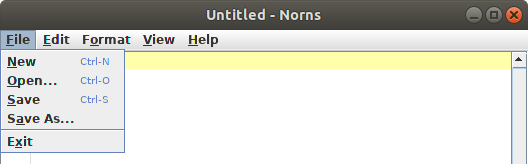
\includegraphics[width = \textwidth]{FileMenu}
\begin{itemize}
  \item \textbf{New:} Létre lehet hozni egy új dokumentumot.
  \item \textbf{Open...:} Meglehet nyitni egy új doksit.
  \item \textbf{Save:} Mikor csak simán menteni szeretnénk egy meglévő fájlra.
  \item \textbf{Save As...:} Mikor máshogyan akarunk elmenteni egy fájlt.
  \item \textbf{Exit:} Ha kiszeretnénk lépni a programból.
\end{itemize}

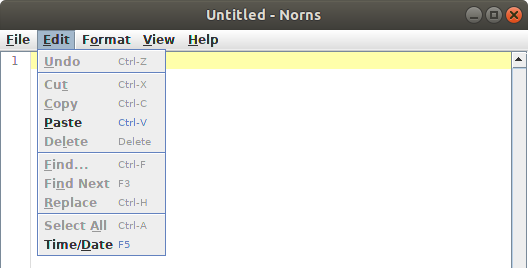
\includegraphics[width = \textwidth]{EditMenu}
\begin{itemize}
  \item \textbf{Undo:} Viszavonást lehet vele megvalósítani.
  \item \textbf{Cut:} Kitudunk vágni egy darabot a szövegből.
  \item \textbf{Copy:} Tudunk másolni szöveget.
  \item \textbf{Paste:} Betudunk illeszteni egy szöveget.
  \item \textbf{Delete:} Kitudjuk törölni a kijelölt részt.
  \item \textbf{Find...:} Megnyit egy keresési panelt, ahol tudunk keresni szöveget.
  \item \textbf{Find Next:} A következő egyező részt kijelöli.
  \item \textbf{Replace:} Kicseréli a következő olyan szöveget, ami egyezik.
  \item \textbf{Select All:} Kiválasztja az egész szöveget.
  \item \textbf{Time/date:} Beszúrja az aktuális dátumot ilyen formában.
  \begin{lstlisting}
    Sun Nov 25 09:24:51 CET 2018
  \end{lstlisting}
\end{itemize}

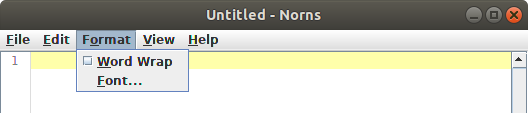
\includegraphics[width = \textwidth]{FormatMenu}
\begin{itemize}
  \item \textbf{Word Wrap:} Megtöri a szöveget.
  \item \textbf{Font:} Előhozza a szöveg stílusának beállítását.
\end{itemize}

\begin{center}
  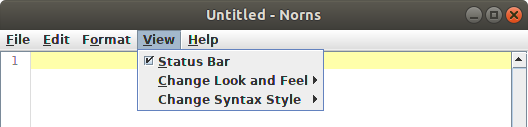
\includegraphics[width = \textwidth]{ViewMenu}
  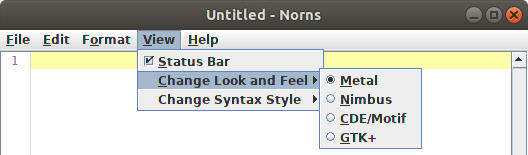
\includegraphics[width = \textwidth]{ViewLookMenu}
  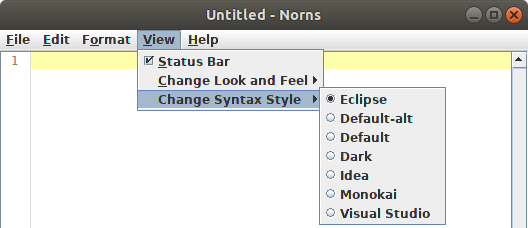
\includegraphics[width = \textwidth]{ViewSyntaxMenu}
\end{center}
\begin{itemize}
  \item \textbf{Status Bar:} Eltünteti vagy megjeleníti a Status Bar-t.
  \item \textbf{Change Look and Feel:} Kilehet választani a GUI kinézetét.
  \item \textbf{Change Syntax Style:} Meglehet változtatni a szintaxis színezést.
\end{itemize}

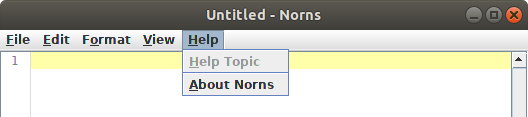
\includegraphics[width = \textwidth]{HelpMenu}
\begin{itemize}
  \item \textbf{Help Topic:} Ha lenne weblap hozzá itt lehetne elérni.
  \item \textbf{About Norns:} Egy kis szöveget ír ki.
\end{itemize}

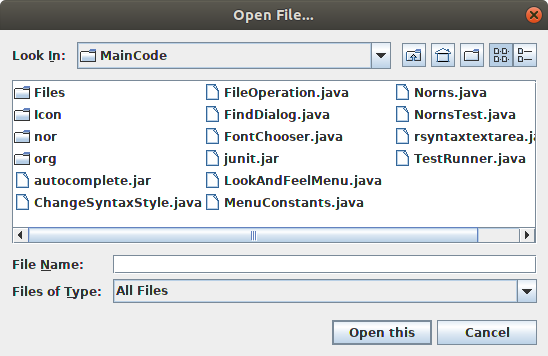
\includegraphics[width = \textwidth]{OpenFile}
Ha megszeretnénk nyitni egy fájlt vagy elmenti másképp, akkor egy ilyen ablakot
fogunk kapni. \\

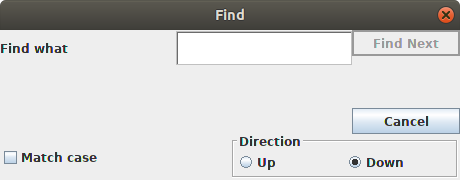
\includegraphics[width = \textwidth]{FindMenu}
Mikor keresni szeretnénk egy szót, de nem akarjuk kicserélni csak megtalálni,
akkor egy ilyen ablakot kapunk.\\

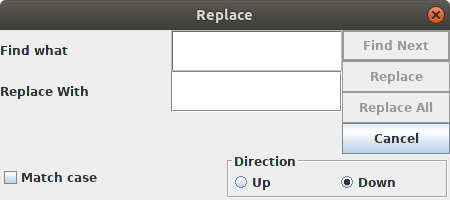
\includegraphics[width = \textwidth]{FindReplace}
Ha szeretnénk keresni, de azt ki is szeretnénk cserélni.\\

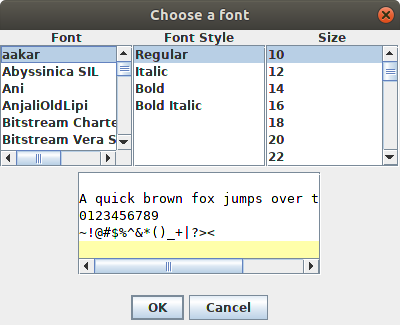
\includegraphics[width = \textwidth]{Font}
Itt kitudjuk választani a szöveg:
\begin{itemize}
  \item Stílusát.
  \item Formázását.
  \item Méretét.
\end{itemize}
És még emellé van egy kis szövegünk is, amin látszik, hogy mit változtattunk.\\

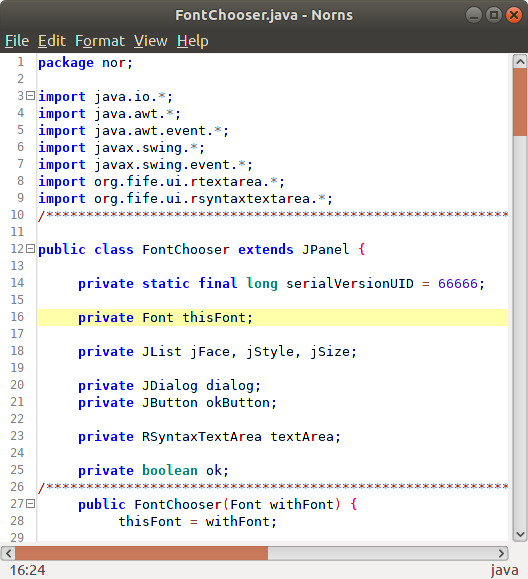
\includegraphics[width = \textwidth]{GTKLook}
Ha megváltoztatjuk a GUI kinézetét pl.: GTK+ kinézetűre. \\

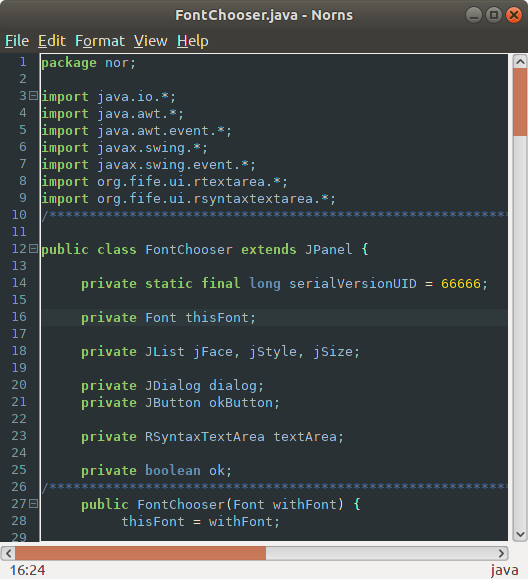
\includegraphics[width = \textwidth]{DarkSyntax}
Ha megváltoztatjuk a szintaxis színezését mondjuk a Dark-ra. \\

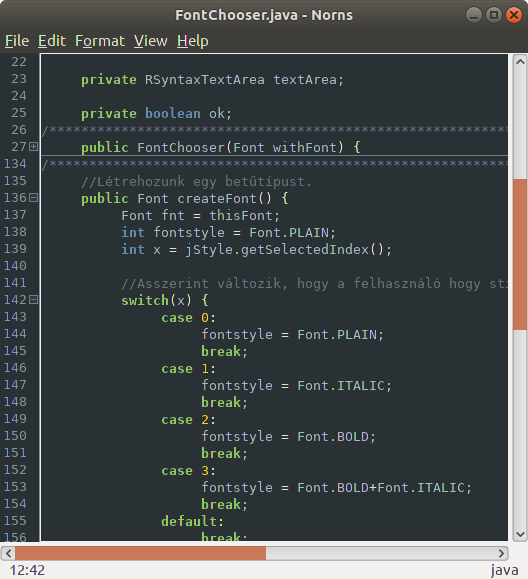
\includegraphics[width = \textwidth]{Folding}
Ha használjuk az összecsukó funkciót, akkor monjuk ilyen függvényekt lehet
összecsukni és, akkor az nem látszik.

\newpage
\section*{Megvalósítás:}
A felhasznált eszközök:
\begin{itemize}
  \item \textbf{Operációs rendszer:} Linux
  \item \textbf{Szövegszerkesztő:} Atom
  \item \textbf{Dokumentációhoz használt eszköz:} Latex
\end{itemize}

A feladat megoldása körülbelül 20-25 órát vett igénybe. 

\end{document}
